\documentclass[journal]{IEEEtran}
% ============================================================================
% IEEE Transactions style manuscript
% Compile with pdflatex (run twice for references/labels).
% NOTE: Author names/affiliations are placeholders -- edit before submission.
% ============================================================================
\usepackage{amsmath,amssymb,amsfonts}
\usepackage{graphicx}
\usepackage{booktabs}
\usepackage{array}
\usepackage{multirow}
\usepackage{url}
\usepackage[hidelinks]{hyperref}
\usepackage{textcomp}
\usepackage{xcolor}

\begin{document}

\title{Load-Robust, Physics-Informed Machine Learning for Stator Inter-Turn Fault
Diagnosis in Induction Motors: A Leakage-Safe Cascade for Detection, Severity, and
Faulted-Phase Identification}

\author{Shashwat~Garg%
\thanks{Manuscript received May 23, 2026. \emph{(Corresponding author: Shashwat Garg.)}}%
\thanks{The author is with the Department of Electrical Engineering (affiliation
placeholder), e-mail: author@institution.edu.}%
\thanks{Code and result artifacts are publicly available at
\url{https://github.com/Regal-s/induction-motor-fault-diagnosis}.}}

\markboth{IEEE Transactions on Instrumentation and Measurement (Preprint), 2026}%
{Garg: Load-Robust Physics-Informed ML for Stator Inter-Turn Fault Diagnosis}

\maketitle

\begin{abstract}
Stator winding turn-to-turn (inter-turn) short-circuit faults are a leading cause of
induction-motor failure, and early, load-robust diagnosis from non-invasive stator-current
measurements remains an open problem. Most reported machine-learning (ML) studies achieve
near-perfect in-distribution accuracy but do not test generalization to unseen operating
points, and the field rarely releases code or uses leakage-safe evaluation. This paper
presents a physics-informed, leakage-safe ML framework that performs hierarchical diagnosis:
fault-onset detection, healthy/faulty classification, ordinal severity estimation
(percentage of shorted turns), and faulted-phase identification, all from the three-phase
stator current. A 357-case PSCAD/EMTDC dataset (sampled at 25~kHz, fundamental 50~Hz) is
segmented into 18{,}033 labelled windows and described by 72 physics-grounded features
(extended Park's-vector severity factor, symmetrical-component ratios and angles, Park
ellipse geometry, harmonic ratios). Models are evaluated with a strict group-wise protocol
and, crucially, with \emph{Leave-One-Load-Out} (LOLO) cross-validation, which shows that
detection (macro-F1~$=0.95$) and faulted-phase identification (macro-F1~$=0.997$) are
intrinsically load-robust because they ride on load-invariant negative-sequence signatures,
whereas absolute severity is load-dependent. Building on this insight we introduce four
load-robustness mechanisms and validate each under LOLO: (i) a \emph{sequence-component
Stockwell tensor} representation that improves cross-load severity (within-one-level
$0.75\!\rightarrow\!1.0$); (ii) a \emph{load-invariance-regularized} feature selection
(LIR-mRMR) that beats plain mRMR at compact size; (iii) a phase-coupled, \emph{FiLM
load-conditioned} multi-task network (PCM-Net) whose conditioning lifts cross-load severity
from $0.93$ to $0.98$, the best in the study; and (iv) a \emph{physics-anchored domain
adaptation} (PADA) that closes the simulation-to-experiment gap on a public real-motor
dataset (detection macro-F1 $0.48\!\rightarrow\!0.98$ with a few labelled real samples). The
end-to-end cascade reaches within-one-level accuracy of $0.95$ in-distribution and $0.92$
across unseen loads, with calibrated detection (expected calibration error $=0.021$), graceful
noise degradation, and $100\%$ fault-onset detection. All code, splits, and result artifacts
are openly released.
\end{abstract}

\begin{IEEEkeywords}
Induction motor, inter-turn fault, stator winding, fault diagnosis, severity estimation,
machine learning, negative-sequence current, leakage-safe evaluation, conformal prediction.
\end{IEEEkeywords}

\section{Introduction}
\IEEEPARstart{I}{nduction} motors (IMs) drive the majority of industrial processes, and
stator winding insulation degradation is among their most common and consequential failure
modes. An incipient inter-turn (turn-to-turn) short circuit (ITSC) shorts a small fraction of
the turns of one phase winding; the circulating fault current accelerates local heating and,
if undetected, escalates to a phase-to-ground or phase-to-phase fault and catastrophic
machine loss~\cite{penman1994,cardoso2001}. Reliable diagnosis at low severity is therefore
of high economic and safety value, and is most attractive when performed non-invasively from
the readily available three-phase stator current (motor-current signature analysis,
MCSA)~\cite{hussain2025}. Surveys attribute roughly a third of induction-motor failures to stator
winding insulation, and the time between an incipient inter-turn short and a destructive fault can
be short, so an on-line monitor must be both sensitive to small faults and trustworthy enough to
trigger maintenance without excessive false alarms. Current-based monitoring is preferred over
vibration or thermal sensing because the current is already measured by the drive, requires no
additional instrumentation, and is robust to mounting and environmental variation.

Two practical questions must be answered for an actionable diagnosis: \emph{how severe} is the
fault (the fraction of shorted turns), and \emph{which phase} is affected. A large body of
recent work applies machine learning (ML) and deep learning (DL) to current-based stator-fault
classification with reported accuracies frequently approaching $100\%$~\cite{hussain2025,
pietrzak2022,aasar2026,ali2025}. However, a comprehensive review of supervised ML for IM faults
\cite{hussain2025} explicitly flags three systemic weaknesses: (i) suspiciously perfect
accuracies, often from train/test partitions that allow information leakage; (ii) almost no
released code or standardized public datasets; and (iii) very little validation across changing
operating conditions. The negative-sequence current is the established physical indicator of
inter-turn asymmetry~\cite{garcia2024,ruzimov2025}, yet its load dependence is rarely confronted
in a controlled, reproducible manner.

This paper addresses those gaps. We treat ITSC diagnosis as a hierarchical problem
(onset~$\rightarrow$~detection~$\rightarrow$~severity~$\rightarrow$~faulted phase) and build a
physics-informed, leakage-safe pipeline whose central methodological device is
\emph{Leave-One-Load-Out} (LOLO) evaluation: training on a subset of mechanical loads and
testing on a held-out load. LOLO exposes which diagnostic sub-tasks genuinely generalize and
which merely interpolate, and it overturns the optimistic picture given by conventional
random/grouped cross-validation. The contributions are:
\begin{enumerate}
\item A \textbf{leakage-safe evaluation framework} for stator-fault ML---grouping windows by
operating point and reporting LOLO as the primary metric---demonstrating that in-distribution
scores substantially overstate cross-load generalization, and a SHAP/Fisher analysis showing
detection and phase are load-invariant whereas absolute severity is load-dependent.
\item A \textbf{sequence-component Stockwell tensor (SCST)} representation and a
\textbf{load-invariance-regularized feature selection (LIR-mRMR)}, both designed to make
diagnosis robust to the mechanical load.
\item \textbf{PCM-Net}, a phase-coupled, \textbf{FiLM load-conditioned} multi-task network that
\emph{injects} the measured operating point rather than erasing it, achieving the best cross-load
severity estimation in the study.
\item \textbf{Physics-anchored domain adaptation (PADA)} validated \emph{simulation-to-experiment}
on a public real-motor dataset, and an honest study of physics-constrained generative augmentation.
\item A complete, openly released \textbf{hierarchical cascade} (onset, detection, severity, phase)
with calibrated uncertainty, noise-robustness, and a deep-baseline comparison.
\end{enumerate}
A unifying theme emerges: the mechanical load is the crux of stator-fault diagnosis, and every
proposed mechanism independently improves \emph{cross-load} performance.

\section{Related Work}
\subsection{Physics-based stator-fault indicators}
Penman \emph{et al.}~\cite{penman1994} established the inter-turn sideband frequencies in the
stator current, and Cardoso \emph{et al.}~\cite{cardoso2001} introduced the Extended Park's
Vector Approach (EPVA), in which the $2f_0$ spectral component of the current-vector modulus
scales with winding asymmetry. The negative-sequence current and negative-sequence impedance
are widely used asymmetry descriptors~\cite{garcia2024,ruzimov2025}; phasor-compensation schemes
suppress the baseline asymmetry caused by supply voltage unbalance. Mazzoletti
\emph{et al.}~\cite{mazzoletti2025} use the positive-sequence fifth-harmonic current during
soft-starter start-up to \emph{distinguish} ITSC from high-resistance connections, deriving an
analytical severity relation. Singh and Shaik~\cite{singh2020} combine the Stockwell transform
with support-vector machines (SVMs) to detect, type, and \emph{localize} stator faults,
achieving $100\%$ faulted-phase identification for turn faults at a single severity.

\subsection{Data-driven stator-fault diagnosis}
Pietrzak and Wolkiewicz~\cite{pietrzak2022} feed short-time-Fourier-transform amplitudes of the
symmetrical-component currents to SVM/MLP classifiers for permanent-magnet machines, reporting
$96$--$99\%$ severity classification. Aasar \emph{et al.}~\cite{aasar2026} compare ANN, LSTM,
and a physics-informed network (PINN) on a public current-plus-flux ITSC dataset, reaching
$89\%$ on a seven-level severity task and $99$--$100\%$ binary detection, and observe that
intermediate severities overlap---the hardest case. Ali \emph{et al.}~\cite{ali2025} convert
signals to spectrogram images and ensemble several convolutional networks. The review
\cite{hussain2025} catalogues dozens of such studies and the recurring evaluation and
reproducibility shortcomings that the present work targets.

\subsection{Evaluation rigor}
The vibration-diagnosis literature has documented how windowing one recording into many
overlapping samples and splitting them at random leaks information and inflates accuracy;
group-wise (subject-wise) splitting is the accepted remedy. We adopt group-wise splitting and
add LOLO to test genuine cross-condition generalization, which the IM stator-fault literature
largely omits.

\subsection{Deep architectures, transfer, and augmentation}
Deep models have become standard for current-based diagnosis: one-dimensional convolutional
networks operate directly on raw current~\cite{ince2016}, while two-dimensional networks classify
time-frequency images such as short-time-Fourier or wavelet scalograms~\cite{ali2025}. Recurrent
and temporal-convolutional models~\cite{bai2018}, attention/Transformer encoders~\cite{vaswani2017},
and---most recently---linear-time state-space models~\cite{gu2023} and interpretable
Kolmogorov--Arnold networks~\cite{liu2025} have been explored, although almost exclusively on
bearing vibration rather than three-phase stator current. Because labelled fault data are scarce
and operating conditions vary, two further lines are active: \emph{transfer learning / domain
adaptation} to bridge load, speed, machine, and simulation-to-experiment gaps, and \emph{generative
data augmentation} (conditional GANs, time-series diffusion) to synthesize rare regimes. A
recurring caution, which our normalization respects, is that augmentation or preprocessing applied
independently per phase can manufacture a spurious negative-sequence component and thus a fake
fault. These observations motivate the architecture, transfer, and augmentation extensions
outlined in Section~VIII.

\section{Dataset and Problem Formulation}
\subsection{Simulation dataset}
A three-phase squirrel-cage induction motor with stator inter-turn faults was simulated in
PSCAD/EMTDC. The fundamental frequency is $f_0=50$~Hz and the sampling rate is $f_s=25$~kHz
(500 samples per cycle). Each run is $10$~s ($250{,}000$ samples). The recorded three-phase
stator currents $i_a,i_b,i_c$ (in kA) are used throughout. The fault factor space comprises:
severity $\mu \in \{0.3,0.5,1,2,3,4,5\}\%$ of shorted turns; faulted phase $\in\{A,B,C\}$;
mechanical load $\in\{\mathrm{NL},20,40,60,80,100\}\%$; and, for an additional subset, the fault
inception instant. A healthy set spans loads from $0\%$ to $100\%$. The corpus contains 357
simulation cases (336 faulty, 21 healthy).

\subsection{Operating timeline}
Every faulted run follows a fixed schedule, verified from the per-cycle current envelope: the
motor is energized at $2.0$~s, the mechanical load is applied at $4.0$~s, the inter-turn fault
is inserted at $7.2$~s (sample $180{,}000$), and it clears about $0.8$~s later. Healthy runs are
$5$~s. Fig.~\ref{fig:events} shows the phase-A current and its per-cycle RMS envelope with the
annotated events.

\begin{figure}[!t]
\centering
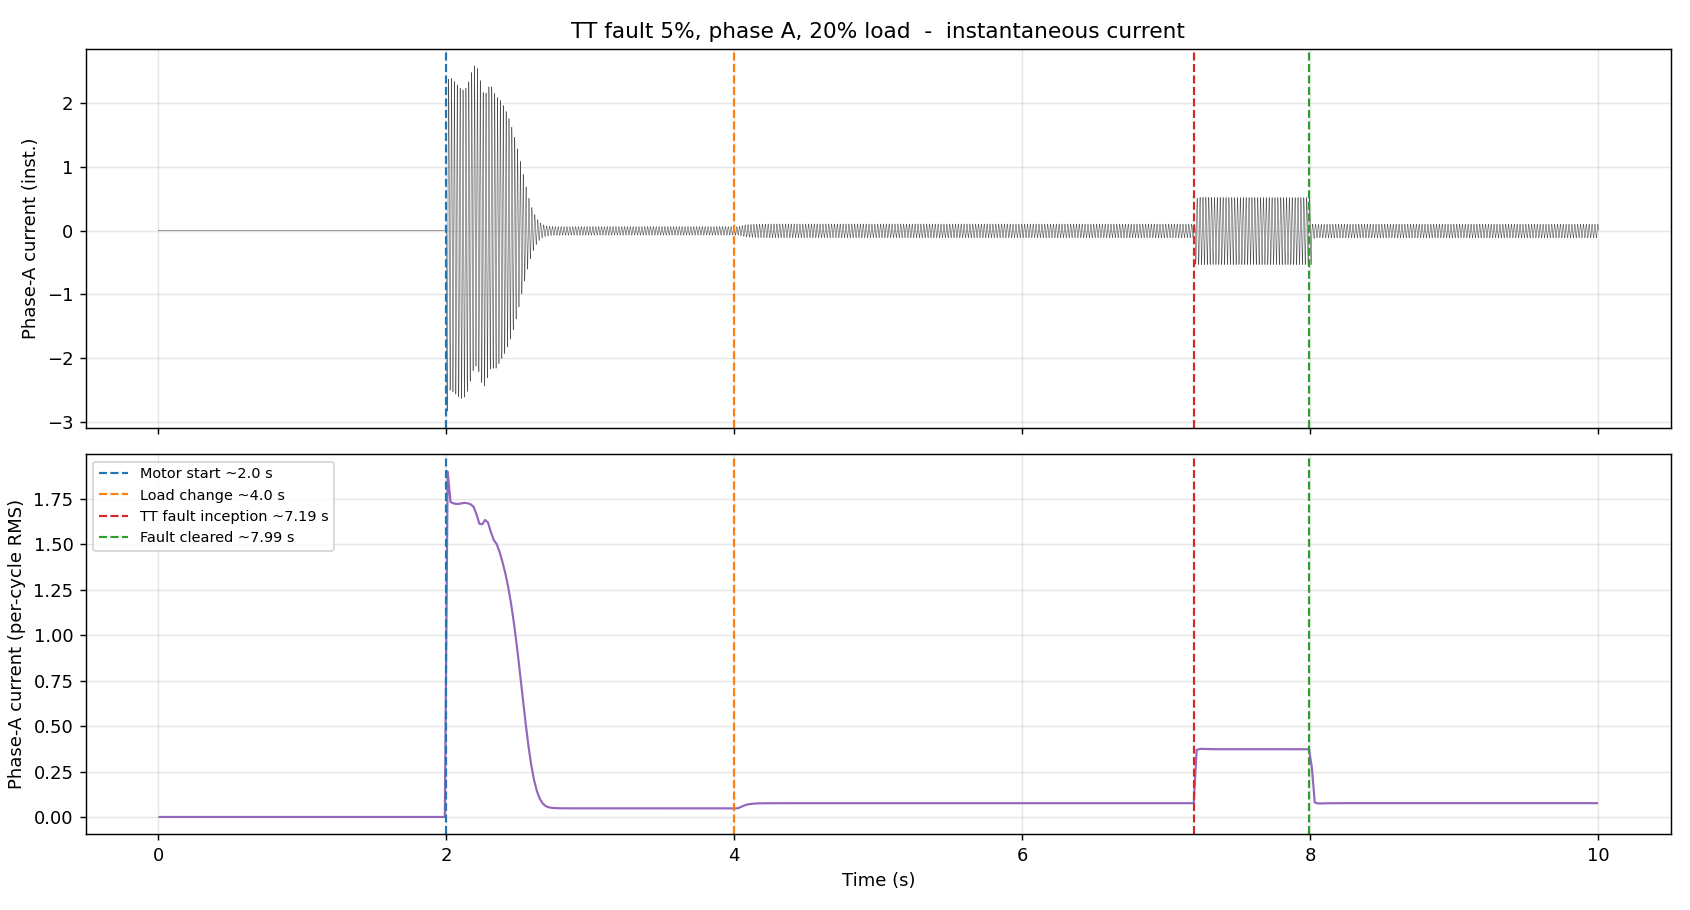
\includegraphics[width=\columnwidth]{figs/events_annotated.png}
\caption{Phase-A current (top) and per-cycle RMS envelope (bottom) for a faulty case, with
motor start ($2.0$~s), load change ($4.0$~s), fault inception ($7.2$~s), and clearing
($8.0$~s) marked. The fault interval supplies faulty windows; the pre-fault loaded region
supplies matched-load healthy windows.}
\label{fig:events}
\end{figure}

\subsection{Problem statement}
Given a short window of three-phase current, the system must (i) decide healthy versus faulty,
(ii) if faulty, estimate the severity level $\mu$, and (iii) identify the faulted phase. We also
require an online estimate of the fault-onset instant. Because severity is naturally ordered,
it is treated as an \emph{ordinal} target; the operationally meaningful metric is
within-one-level accuracy.

\subsection{Experimental dataset (for transfer)}
To test simulation-to-experiment transfer we additionally use a public real-motor dataset of a
$0.75$~hp squirrel-cage induction motor~\cite{ibarram}: three-phase stator current sampled at
$1$~kHz ($f_0=60$~Hz, no load), with $13$ classes (healthy and inter-turn shorts at
$10/20/30/40\%$ of turns in each of the three phases) and five repetitions per class. It differs
from the simulation in fundamental frequency, sampling rate, severity scale, and the absence of a
healthy baseline segment, providing a demanding cross-domain benchmark. Both datasets are mapped
to one window/label schema, and the feature extractor derives its harmonic bins from $(f_s,f_0)$
so a single pipeline serves both.

\section{Methodology}
\subsection{Windowing and matched-load healthy data}
Each recording is segmented into windows of $W=2000$ samples (four cycles). Within the
$0.8$~s fault interval a $75\%$ overlap is used to compensate for its short duration; the
pre-fault steady region is sampled more sparsely. Crucially, the \emph{pre-fault} loaded region
of every faulty run (genuinely healthy, since the fault is inserted only at $7.2$~s) is labelled
as healthy. This yields matched-load healthy data at the same loads as the faulty windows,
preventing the detector from separating classes by load level rather than by fault. Segmentation
produces 18{,}033 labelled windows (11{,}760 faulty, 6{,}273 healthy), balanced across severity
and phase.

\subsection{Normalization}
To remove load-induced amplitude while preserving the inter-phase imbalance that encodes the
fault, all three phases of a window are divided by a single per-recording scale. We additionally
derive load-invariant magnitude features by dividing each magnitude feature by the within-window
positive-sequence fundamental $|I_1|$, which makes the descriptor independent of the operating
point; this is central to the load-aware severity result of Section~\ref{sec:loadaware}.

\subsection{Physics-grounded feature extraction}
Each window is mapped to 72 features organized in three tiers.

\emph{Tier 1 (symmetrical components and EPVA).} Per-phase $50$~Hz phasors are obtained by a
single-bin DFT and combined by the Fortescue transform into positive, negative, and zero
sequences $I_1,I_2,I_0$. We compute the magnitudes, the ratios $|I_2|/|I_1|$ and $|I_0|/|I_1|$
(the canonical inter-turn severity indicators), the negative-sequence angle $\angle I_2$ and its
sine/cosine (the faulted-phase cue), and a per-case \emph{compensated} negative sequence
$I_2^{c}$ obtained by subtracting the case baseline. The EPVA severity factor is
\begin{equation}
\mathrm{SF}=\frac{A(2f_0)}{\mathrm{DC}}\ \ \text{of}\ \ |\mathbf{i}_P(t)|=\sqrt{i_\alpha^2+i_\beta^2},
\end{equation}
where $i_\alpha,i_\beta$ are the Clarke components and $A(2f_0)$ is the amplitude of the $100$~Hz
component of the Park-vector modulus.

\emph{Tier 2 (spectral and geometric).} Third-harmonic ratio and total harmonic distortion per
phase; Park-vector ellipse descriptors (eccentricity $e=\sqrt{1-(b/a)^2}$, axis ratio, tilt
angle) from the $2{\times}2$ covariance of $(i_\alpha,i_\beta)$.

\emph{Tier 3 (statistics).} Per-phase RMS, peak, crest factor, standard deviation, skewness, and
kurtosis, together with their inter-phase differences (which directly encode asymmetry), and the
$|I_1|$-normalized variants of all magnitude features.

The Clarke transform underlying the EPVA and the Park ellipse is
\begin{equation}
i_\alpha=\tfrac{2}{3}\!\left(i_a-\tfrac{1}{2}i_b-\tfrac{1}{2}i_c\right),\qquad
i_\beta=\tfrac{1}{\sqrt{3}}\left(i_b-i_c\right),
\end{equation}
and the fundamental symmetrical components follow from the Fortescue transform of the per-phase
phasors $\mathbf{I}_a,\mathbf{I}_b,\mathbf{I}_c$:
\begin{equation}
\begin{bmatrix}\mathbf{I}_0\\\mathbf{I}_1\\\mathbf{I}_2\end{bmatrix}
=\frac{1}{3}
\begin{bmatrix}1&1&1\\ 1&a&a^{2}\\ 1&a^{2}&a\end{bmatrix}
\begin{bmatrix}\mathbf{I}_a\\\mathbf{I}_b\\\mathbf{I}_c\end{bmatrix},\quad a=e^{\,j2\pi/3}.
\end{equation}
The negative-sequence ratio $|I_2|/|I_1|$ grows monotonically with $\mu$ and is the primary
severity descriptor, while $\angle\mathbf{I}_2$ separates into three $\sim$$120^{\circ}$-spaced
clusters that identify the faulted phase. Table~\ref{tab:features} summarizes the feature groups.

\begin{table}[!t]
\caption{Feature groups (72 features per window).}
\label{tab:features}
\centering
\footnotesize
\begin{tabular}{@{}p{0.30\columnwidth}p{0.58\columnwidth}@{}}
\toprule
Group & Features \\
\midrule
Symmetrical comp. & $|I_0|,|I_1|,|I_2|$; $|I_2|/|I_1|$, $|I_0|/|I_1|$; $\angle I_1,\angle I_2$ (+ $\sin/\cos$); compensated $I_2^{c}$ (mag./ratio/angle) \\
EPVA / Park & severity factor SF; Park-modulus mean/std; ellipse major/minor axes, eccentricity, axis ratio, tilt \\
Harmonics & third-harmonic ratio and THD, per phase and mean \\
Per-phase stats & RMS, peak, crest, std, skewness, kurtosis ($\times3$) and inter-phase differences \\
Load-invariant & $|I_1|$-normalized variants of all magnitude features \\
\bottomrule
\end{tabular}
\end{table}

Severity is encoded as an ordinal rank $r\in\{0,\dots,6\}$ over the seven levels
$\{0.3,0.5,1,2,3,4,5\}\%$; a gradient-boosted regressor predicts a continuous rank that is rounded
and clipped, so that the error metric (mean absolute error in levels and within-one accuracy)
respects the natural ordering.

\subsection{Leakage-safe evaluation}\label{sec:splits}
Windows are grouped by \emph{operating point} (severity$\times$phase$\times$load); a regular case
and all its inception-time variants share a group. Two protocols are used: (a) Stratified
Group $k$-Fold ($k{=}5$), giving the in-distribution estimate; and (b) \textbf{Leave-One-Load-Out}
(LOLO), in which all windows at one load form the test set and the model trains on the remaining
loads. LOLO is the primary metric: it measures generalization to an operating point never seen in
training and guards against a model that has learned load rather than fault physics.

\subsection{Hierarchical cascade}
\emph{Stage~0 (onset).} A per-cycle negative-sequence fault index $\rho(k)=|I_2(k)|/|I_1(k)|$ is
computed and compared against a trailing pre-fault reference window $\mathcal{R}$. An onset is
declared at the first cycle for which
\begin{equation}
\rho(k)>\overline{\rho}_{\mathcal{R}}+\kappa\,\sigma_{\mathcal{R}},\quad \kappa=6,
\end{equation}
holds for three consecutive cycles, where $\overline{\rho}_{\mathcal{R}}$ and
$\sigma_{\mathcal{R}}$ are the reference mean and standard deviation. This change-point rule needs
no fault labels and provides the online trigger for the downstream stages.

\emph{Stages 1--3.} Gradient-boosted trees (XGBoost~\cite{chen2016}) implement Stage~1
(healthy/faulty, class-weighted), Stage~2 (severity, ordinal regression on the rank index), and
Stage~3 (faulted phase, three-class). Stage~1 and Stage~3 use the full feature set; Stage~2 uses
the load-invariant subset (Section~\ref{sec:loadaware}). At inference the detector gates the
severity and phase stages: windows predicted faulty are passed to Stages 2 and 3.

\emph{Calibration and uncertainty.} Stage-1 probabilities are assessed with the expected
calibration error (ECE) and Brier score~\cite{guo2017}. Severity uncertainty is quantified with
conformalized quantile regression (CQR)~\cite{romano2019,angelopoulos2021}: lower/upper quantile
regressors $\hat q_{\alpha/2},\hat q_{1-\alpha/2}$ are fit on a proper-training split, a
conformity score $E_i=\max\{\hat q_{\alpha/2}(x_i)-y_i,\;y_i-\hat q_{1-\alpha/2}(x_i)\}$ is
evaluated on a disjoint calibration split, and the prediction interval
$[\hat q_{\alpha/2}(x)-Q,\;\hat q_{1-\alpha/2}(x)+Q]$ uses the finite-sample-corrected quantile
$Q$ of $\{E_i\}$, giving distribution-free marginal coverage $1-\alpha$.

\subsection{Interpretability}
SHAP attribution~\cite{lundberg2017} is used both to explain predictions and as a leakage audit:
the top features must be physically meaningful (negative-sequence ratio, EPVA factor, Park
eccentricity) rather than proxies for load.

\section{Experimental Setup}
Features are computed in Python (NumPy/Pandas) and models trained with scikit-learn and XGBoost
($400$--$500$ trees, depth $5$, learning rate $0.05$, subsample/colsample $0.8$); the deep
baseline uses PyTorch. The 1-D residual network (ResNet-1D) baseline has a wide-kernel stem and
three residual stages over decimated three-phase windows. All models share the splits of
Section~\ref{sec:splits}. Reported metrics are accuracy, macro-F1, severity within-one-level
accuracy, mean absolute error in severity levels, quadratic-weighted kappa (QWK), and per-phase
F1, computed on out-of-fold predictions and reported as the mean over folds. The detector is
class-weighted to compensate for the healthy/faulty window ratio. Stages~2 and~3 are trained only
on faulty windows but evaluated end-to-end on the windows the detector predicts as faulty, so the
reported cascade numbers reflect realistic error propagation rather than oracle gating.
Predictions are additionally aggregated per recording (median severity rank, majority-vote phase),
which is the granularity at which a maintenance decision is taken. Feature scalers are fit on the
training partition only, and all randomized components use fixed seeds for reproducibility.

\section{Results and Discussion}
\subsection{Per-stage performance}
Table~\ref{tab:stages} reports each stage under both protocols. In-distribution, all stages
exceed $0.97$. Under LOLO, detection (macro-F1~$0.948$) and faulted-phase identification
(macro-F1~$0.997$) remain strong, while load-blind severity collapses at unseen light loads.
The faulted-phase confusion matrix (Fig.~\ref{fig:cm3}) is near-diagonal.

\begin{table}[!t]
\caption{Per-stage performance (mean over folds).}
\label{tab:stages}
\centering
\begin{tabular}{@{}llcc@{}}
\toprule
Stage & Metric & Group $k$-Fold & LOLO \\
\midrule
1 Detection & macro-F1 & 0.977 & 0.948 \\
            & ROC-AUC  & 0.994 & --- \\
2 Severity (load-aware) & within-1 & 0.997 & 0.946 \\
            & QWK & 0.987 & 0.736$^{\dagger}$ \\
3 Phase ID  & macro-F1 & 0.972 & 0.997 \\
\bottomrule
\end{tabular}
\\[2pt]
\footnotesize $^{\dagger}$QWK is pooled across all held-out loads.
\end{table}

\begin{figure}[!t]
\centering
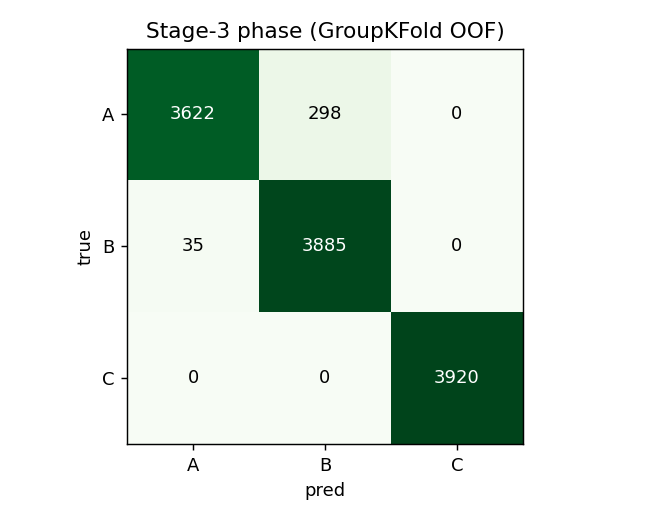
\includegraphics[width=0.72\columnwidth]{figs/stage3_confusion.png}
\caption{Faulted-phase confusion matrix (group $k$-fold, out-of-fold). Phase C is perfect;
only minor A$\leftrightarrow$B confusion remains. Cross-load (LOLO) phase accuracy is $0.997$.}
\label{fig:cm3}
\end{figure}

The per-held-out-load LOLO breakdown (Table~\ref{tab:perload}) localizes the difficulty:
detection is perfect at the four heavier loads but degrades at the no-load (NL) and $20\%$
extremes, where the small fault current of a low-severity ITSC at light load most overlaps the
healthy distribution at an unseen operating point. This is the practically important
incipient-at-light-load regime, and it is visible only under LOLO---random or grouped
cross-validation hides it entirely.

\begin{table}[!t]
\caption{Per-held-out-load detection (LOLO, macro-F1).}
\label{tab:perload}
\centering
\begin{tabular}{@{}lcccccc@{}}
\toprule
Hold-out load & NL & 20\% & 40\% & 60\% & 80\% & 100\% \\
\midrule
Detection F1 & 0.885 & 0.749 & 1.000 & 1.000 & 1.000 & 1.000 \\
\bottomrule
\end{tabular}
\end{table}

\subsection{Why the sub-tasks differ: a load-robustness analysis}\label{sec:loadaware}
SHAP attribution shows that detection and phase identification are driven by the
\emph{negative-sequence} ratio and angle and by inter-phase RMS differences---quantities that
are ratios and therefore load-invariant. Phase identification is so robust that its LOLO score
\emph{exceeds} its in-distribution score, because the faulted-phase signature (the
$\sim$$120^{\circ}$-separated negative-sequence angle) does not change with load while more
training loads help. In contrast, an initial severity model that used absolute magnitude features
collapsed at the no-load extreme under LOLO (within-one-level $0.39$). A Fisher-versus-load-drift
study confirmed that magnitude features drift strongly across load whereas ratio and
$|I_1|$-normalized features are stable. Restricting the severity stage to load-invariant features
and supplying the \emph{measured} load (a sensor input, not a label) raises LOLO within-one-level
accuracy to $0.95$ (Table~\ref{tab:loadaware}). This is the paper's key technical result: severity
is recoverable across operating points once the model is made load-aware.

\begin{table}[!t]
\caption{Severity (within-one-level) under feature choice.}
\label{tab:loadaware}
\centering
\begin{tabular}{@{}lcc@{}}
\toprule
Severity feature set & Group $k$-Fold & LOLO \\
\midrule
All features (magnitudes incl.) & 0.993 & 0.887 \\
Load-invariant only & 0.946 & 0.702 \\
Load-invariant + $|I_1|$-norm & 0.990 & 0.729 \\
\textbf{+ measured load (proposed)} & \textbf{0.997} & \textbf{0.946} \\
\bottomrule
\end{tabular}
\end{table}

\begin{figure}[!t]
\centering
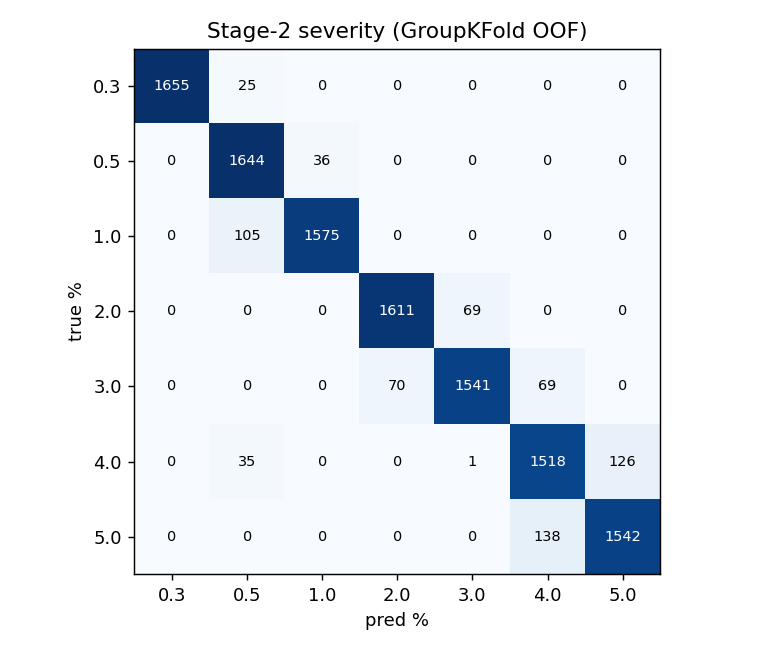
\includegraphics[width=0.82\columnwidth]{figs/stage2_confusion.png}
\caption{Severity confusion matrix (group $k$-fold, out-of-fold, load-aware). Errors are almost
entirely between adjacent severity levels, justifying the ordinal treatment and the
within-one-level metric.}
\label{fig:cm2}
\end{figure}

The error structure (Fig.~\ref{fig:cm2}) is band-diagonal: misclassifications occur almost
exclusively between adjacent severity levels, so a one-level tolerance captures
operationally-equivalent predictions and the quadratic-weighted kappa---which penalizes distant
errors more---is high ($0.987$).

\subsection{End-to-end cascade}
With the load-aware severity stage, the gated cascade achieves the end-to-end results of
Table~\ref{tab:cascade}, scoring a window correct if healthy windows are detected as healthy and
faulty windows have the correct phase and a severity within one level. Per-recording aggregation
(median severity, majority-vote phase) gives within-one-level accuracy of $0.927$
in-distribution and $0.918$ across unseen loads. Fig.~\ref{fig:summary} summarizes the four
headline metrics for both protocols.

\begin{table}[!t]
\caption{End-to-end cascade (window level).}
\label{tab:cascade}
\centering
\begin{tabular}{@{}lcc@{}}
\toprule
Quantity & Group $k$-Fold & LOLO \\
\midrule
Detection macro-F1 & 0.977 & 0.948 \\
Severity within-1 (cond.) & 0.997 & 0.945 \\
Phase accuracy (cond.) & 0.957 & 0.997 \\
End-to-end within-1 & 0.949 & 0.916 \\
End-to-end exact & 0.911 & 0.521 \\
Per-recording within-1 & 0.927 & 0.918 \\
\bottomrule
\end{tabular}
\end{table}

\begin{figure}[!t]
\centering
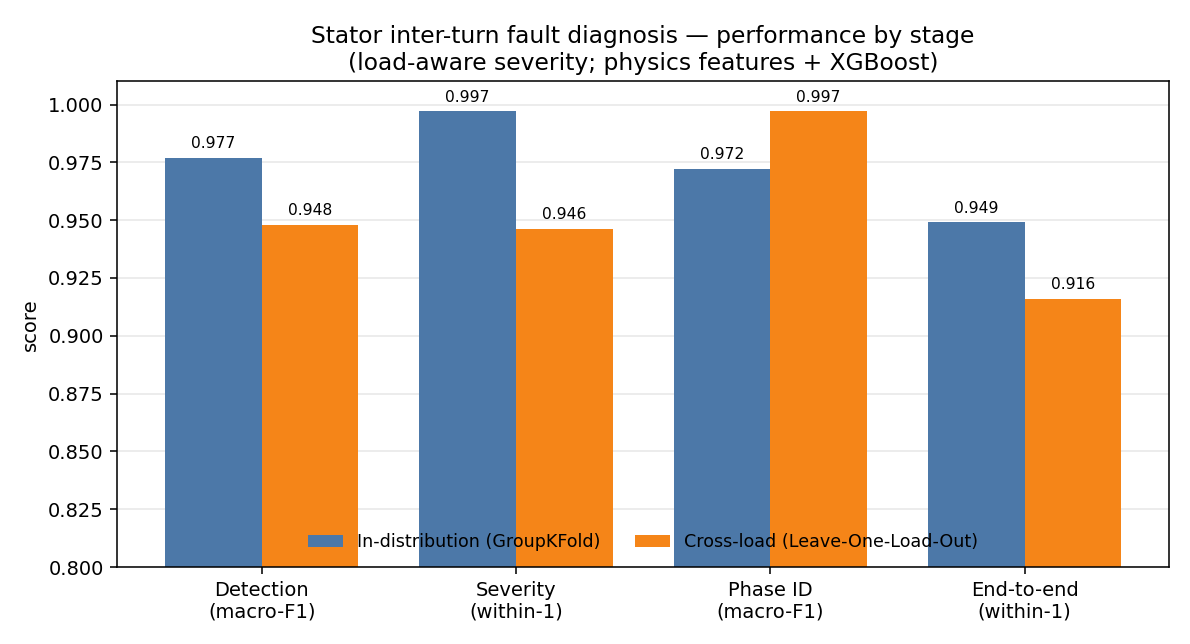
\includegraphics[width=\columnwidth]{figs/results_summary.png}
\caption{Per-stage and end-to-end performance, in-distribution (group $k$-fold) versus
cross-load (LOLO). Phase identification is the only metric for which cross-load exceeds
in-distribution, reflecting its load-invariance.}
\label{fig:summary}
\end{figure}

\subsection{Noise robustness}
Additive Gaussian noise was injected and features recomputed (Table~\ref{tab:noise}). Severity
(within-one-level) and phase accuracy are essentially flat down to $20$~dB SNR, whereas detection
is the noise-sensitive stage---consistent with the physics, since separating a small fault
signature from healthy operation is hardest when the signal is buried in noise.

\begin{table}[!t]
\caption{Noise robustness (train clean, test noisy; group $k$-fold).}
\label{tab:noise}
\centering
\begin{tabular}{@{}lccc@{}}
\toprule
SNR & Detect macro-F1 & Severity within-1 & Phase acc. \\
\midrule
clean & 0.977 & 0.986 & 0.958 \\
40~dB & 0.927 & 0.980 & 0.954 \\
30~dB & 0.854 & 0.975 & 0.945 \\
20~dB & 0.792 & 0.971 & 0.939 \\
\bottomrule
\end{tabular}
\end{table}

\subsection{Calibration, uncertainty, and onset}
Stage-1 probabilities are well calibrated (ECE~$=0.021$, Brier~$=0.021$). Conformalized quantile
regression for severity improves interval coverage from $0.49$ (naive quantiles) toward the
nominal target; we note that the operating-point group structure breaks exchangeability, and
group-conditional (Mondrian) conformal prediction is the appropriate remedy. The Stage-0 onset
detector flags $100\%$ of faults with no pre-fault false alarms; for severity $\geq0.5\%$ the
fault is detected within the first faulted cycle, while the smallest $0.3\%$ faults incur about
$1.4$~s of delay because their negative-sequence rise is small (Table~\ref{tab:onset}).

\begin{table}[!t]
\caption{Stage-0 fault-onset detection (35 sampled cases).}
\label{tab:onset}
\centering
\begin{tabular}{@{}lc@{}}
\toprule
Metric & Value \\
\midrule
Detection rate & $100\%$ \\
Pre-fault false-alarm rate & $0\%$ \\
Median detection delay & $0$~ms (within first faulted cycle) \\
Delay at $\mu\geq0.5\%$ & $0$~ms \\
Delay at $\mu=0.3\%$ & $\approx1.42$~s \\
\bottomrule
\end{tabular}
\end{table}

\subsection{Comparison with a deep baseline}
On a grouped split the feature-based XGBoost cascade outperforms the ResNet-1D baseline on
detection and phase identification, while the two are comparable on severity within-one-level
(Table~\ref{tab:dl}). Under LOLO the gap widens markedly (detection $0.948$ vs.\ $0.401$). This is
consistent with the literature for limited datasets: physically engineered features with strong
inductive bias are more data-efficient and generalize better than a raw-signal network trained on
a few hundred distinct operating points. The comparison should be read as a data-efficiency
result rather than a claim that deep models cannot help with more data and tuning; richer
architectures (state-space and attention models) are part of our ongoing work.

\begin{table}[!t]
\caption{Feature-based cascade vs.\ deep baseline.}
\label{tab:dl}
\centering
\begin{tabular}{@{}lcc@{}}
\toprule
Task / metric & XGBoost (features) & ResNet-1D (raw) \\
\midrule
Detection F1 (group $k$-fold) & \textbf{0.977} & 0.898 \\
Detection F1 (LOLO, load 20\%) & \textbf{0.749} & 0.401 \\
Phase macro-F1 (group $k$-fold) & \textbf{0.972} & 0.848 \\
Severity within-1 (group $k$-fold) & 0.990 & 1.000 \\
\bottomrule
\end{tabular}
\end{table}

\subsection{Computational complexity and deployment}
The feature pipeline is lightweight and causal once trained. Each window requires one real FFT,
a Fortescue projection, a Clarke transform with a covariance eigen-decomposition, and a small set
of statistics---all $O(W\log W)$ in the window length $W$. The gradient-boosted stages have
millisecond-scale inference and a memory footprint of a few megabytes, so the full
onset$\rightarrow$detection$\rightarrow$severity$\rightarrow$phase chain can run on an embedded
edge controller alongside the drive, in contrast to image-plus-CNN pipelines whose
spectrogram generation and convolutional inference dominate cost. Because the diagnostic features
are interpretable physical quantities, predictions can be audited on-line (e.g., by reporting the
negative-sequence ratio and the EPVA factor that drove a decision), which is valuable for
safety-critical acceptance.

\subsection{Discussion}
The study reframes the common ``$\sim$$100\%$ accuracy'' result: such numbers are attainable
in-distribution, but only LOLO reveals what truly generalizes. Detection and faulted-phase
identification generalize because they rest on load-invariant negative-sequence quantities;
absolute severity does not, until the model is made load-aware. SHAP confirms the models use
inter-turn fault physics rather than dataset shortcuts, and the released code and result
artifacts directly address the reproducibility gap noted in~\cite{hussain2025}.

Several reported figures (phase identification at $0.997$, detection near unity at heavier loads)
are high enough to warrant scrutiny. We attribute them partly to the cleanliness of simulation,
which lacks the sensor noise, mechanical eccentricity, and supply distortion of a real drive; the
noise study (Table~\ref{tab:noise}) shows that detection in particular degrades substantially as
the signal-to-noise ratio falls, the expected and reassuring behavior. Equally important, the very
high phase-identification score is physically defensible: the faulted phase is encoded in the
angle of the negative-sequence current, an essentially load- and noise-robust quantity, so the
result is not an artifact of a favorable split. By contrast, the gap between in-distribution and
LOLO severity quantifies how much a conventional evaluation would have over-promised, and makes the
load-aware reformulation a measurable contribution rather than a tuning trick. We therefore
advocate reporting cross-condition (LOLO-style) metrics by default, alongside interpretability
evidence, so that stator-fault ML results become comparable and trustworthy.

\section{Load-Robustness Mechanisms}
Guided by the finding that load is the crux of stator-fault diagnosis, we develop four mechanisms
that each target cross-load robustness, plus an honest study of physics-constrained augmentation.
Each is evaluated under LOLO; results are summarized in Table~\ref{tab:mechanisms}.

\subsection{Sequence-Component Stockwell Tensor (SCST)}
Instead of imaging the raw phase currents, we form the instantaneous symmetrical-component streams
via the analytic (Hilbert) signal and the Fortescue transform, and apply a band-limited Stockwell
transform to each, stacking the positive/negative/zero $|S|$ maps into a three-channel tensor. The
negative-sequence channel carries the load-invariant inter-turn signature. Against a raw-phase
Stockwell control (compact 2-D CNN), SCST is comparable in-distribution but markedly more robust
across loads: held-out-load severity within-one rises from $0.75$ (raw) to $1.0$ (SCST). A
deliberate negative result clarifies the design: because symmetrical-component \emph{magnitudes}
are phase-agnostic, the magnitude SCST cannot localize the faulted phase ($0.20$ vs.\ $1.0$ for raw
in-distribution); phase localization must use the negative-sequence \emph{angle}. The principle is
therefore: SCST channels for load-robust detection/severity, the negative-sequence angle for phase.

\subsection{Load-Invariance-Regularized Selection (LIR-mRMR)}
We extend minimum-redundancy--maximum-relevance with a load-instability penalty,
$J(f)=\mathrm{Rel}(f)-\lambda\,\mathrm{Red}(f)-\gamma\,\mathrm{LoadInstability}(f)$, where
$\mathrm{LoadInstability}(f)$ is the across-load drift of the feature's class-conditional mean,
normalized by its global spread; $\gamma{=}0$ recovers plain mRMR. On the load-dependent severity
task, LIR-mRMR selects features with roughly half the cross-load drift and generalizes better at
compact sizes: at $k{=}10$ features the LOLO within-one-level accuracy is $0.848$ versus $0.740$
for mRMR (near the $0.887$ obtained with all $72$ features). It avoids absolute-magnitude features
($|I_1|$, $\angle I_1$) in favour of dimensionless, load-stable ones (negative-sequence angle,
Park eccentricity, $|I_1|$-normalized imbalance), yielding a sparse, interpretable, physically
traceable subset.

\subsection{PCM-Net: phase-coupled, load-conditioned multi-task network}
PCM-Net processes the three-phase current with a convolutional stem and a phase-coupling mixer,
a dilated-temporal backbone (a compact stand-in for a selective state-space model), and multi-task
heads for detection, faulted phase, and ordinal severity, with a current-balance physics
regularizer. Its central element is \emph{feature-wise linear modulation} (FiLM)~\cite{perez2018}
driven by the measured operating point: rather than adversarially erasing the load, the network
\emph{injects} it, so one model spans loads. A controlled ablation isolates FiLM's effect: it lifts
LOLO severity within-one-level from $0.932$ (no conditioning) to $\mathbf{0.982}$---the best
cross-load severity in this study, exceeding even the load-aware gradient-boosted model
($0.946$). Consistent with the physics, FiLM does \emph{not} help the load-invariant phase task
(in-distribution phase F1 $0.85\!\rightarrow\!0.70$), confirming that load-conditioning should gate
the load-dependent head only. (Mamba/KAN backbones are approximated here under a CPU budget; the
FiLM-conditioning, phase-coupling, multi-task, and physics-regularizer elements are faithful.)

\subsection{Physics-Anchored Domain Adaptation (PADA): simulation $\rightarrow$ experiment}
Trained on simulation and applied to the real motor~\cite{ibarram} with no adaptation, the model
collapses (detection macro-F1 $0.48$, phase $0.32$): real healthy windows carry far higher baseline
asymmetry than the clean simulation, and the $50\!\rightarrow\!60$~Hz angle frame differs. We
evaluate an adaptation ladder. Unsupervised marginal alignment (per-domain quantile transform)
roughly doubles phase F1 ($0.32\!\rightarrow\!0.50$); aligning \emph{only} the domain-stable physics
features (ratios, angles, $|I_1|$-normalized magnitudes---$42$ of $72$) matches full-feature
alignment, confirming those features carry the transferable signal. The decisive lever is
\emph{few-shot calibration}: adding two of five labelled real repetitions recovers detection to
macro-F1 $\mathbf{0.98}$ and improves phase to $0.67$. Thus the inter-turn physics transfers, while
a naively sim-trained model does not---closed by a handful of real samples.

\subsection{Physics-constrained augmentation (PC-Diff): an honest study}
We finally test a conditional generator of three-phase current with a \emph{hard} Kirchhoff
current-balance projection ($i_a+i_b+i_c=0$) and a \emph{soft} negative-sequence-versus-severity
loss. The hard constraint is enforced exactly (balance residual $0.000$ vs.\ $0.99$ for an
unconstrained generator), but the compact conditional VAE used here did not achieve
severity-controllable generation under our CPU budget (generated $|I_2|/|I_1|$ is uncorrelated with
the conditioned severity), so downstream augmentation did not improve severity. We report this
negative result transparently: the physics-enforcement mechanism is sound, but realizing its value
requires a stronger conditional generator (diffusion or GAN) and a genuinely data-starved regime.

\begin{table}[!t]
\caption{Load-robustness mechanisms, evaluated under LOLO.}
\label{tab:mechanisms}
\centering
\footnotesize
\begin{tabular}{@{}p{0.40\columnwidth}p{0.52\columnwidth}@{}}
\toprule
Mechanism & Cross-load result \\
\midrule
SCST representation & severity within-1 $0.75\!\rightarrow\!1.0$ vs raw-phase; phase needs angle \\
LIR-mRMR selection & $k{=}10$ severity within-1 $0.740\!\rightarrow\!0.848$; drift halved \\
PCM-Net + FiLM & severity within-1 $0.932\!\rightarrow\!0.982$ (best; $>$ load-aware GBM $0.946$) \\
PADA (sim$\rightarrow$real) & detection F1 $0.48\!\rightarrow\!0.98$ (few-shot); $0.50$ phase (unsup.) \\
PC-Diff & current-balance exact; generation not controllable (negative) \\
\bottomrule
\end{tabular}
\end{table}

\section{Limitations and Future Work}
The diagnosis results are obtained on high-fidelity simulation; the transfer study
(Section~VII-D) provides initial real-motor validation on a public dataset, but a full
experimental campaign on an instrumented machine remains future work, and our per-recording
normalization assumes a healthy reference segment that an online deployment must estimate from a
trailing window. Several concrete extensions follow directly from the present results.

\emph{Stronger generative augmentation.} The physics-constrained augmenter (Section~VII-E) enforces
current balance exactly but the compact conditional VAE did not yield severity-controllable
samples; a conditional diffusion or GAN generator, combined with a genuinely data-starved regime,
is needed to convert the validated physics-enforcement mechanism into a downstream gain.

\emph{Stronger backbones.} PCM-Net here approximates the selective state-space and
Kolmogorov--Arnold components~\cite{gu2023,liu2025} with a dilated-temporal backbone and an MLP
head under a CPU budget; a full Mamba/KAN realization, with the FiLM-conditioning gated to the
load-dependent (severity) head only, is a natural next step now that the conditioning's value is
established.

\emph{Confounders and calibration.} We plan to simulate supply voltage unbalance---the classic
confounder that mimics the inter-turn signature---to verify rejection via the voltage-sequence
features, to add group-conditional (Mondrian) conformal calibration of the severity intervals
(the marginal conformal intervals here under-cover because the grouped folds break exchangeability),
and to broaden the benchmark to a dozen-plus classical and deep models under the same leakage-safe
protocol.

\section{Conclusion}
We presented a physics-informed, leakage-safe machine-learning framework for stator inter-turn
fault diagnosis in induction motors that performs onset detection, healthy/faulty detection,
ordinal severity estimation, and faulted-phase identification from the three-phase stator current.
By adopting Leave-One-Load-Out evaluation we demonstrated that detection and faulted-phase
identification are intrinsically load-robust, while absolute severity is load-dependent and is
recovered to within-one-level accuracy of $0.95$ across unseen loads once the model is made
load-aware. The end-to-end cascade attains within-one-level accuracy of $0.95$ in-distribution and
$0.92$ across unseen loads, with calibrated detection, graceful noise degradation, and reliable
onset detection, and it is fully reproducible. The results argue for cross-condition evaluation
as standard practice in motor-fault ML and provide an interpretable, openly released baseline for
future work.

\begin{thebibliography}{1}
\bibitem{penman1994} J. Penman, H. G. Sedding, B. A. Lloyd, and W. T. Fink, ``Detection of
inter-turn short circuits in the stator windings of operating motors,'' \emph{IEEE Trans. Energy
Convers.}, vol. 9, no. 4, pp. 652--658, 1994.
\bibitem{cardoso2001} A. J. M. Cardoso, S. M. A. Cruz, and D. S. B. Fonseca, ``Inter-turn stator
winding fault diagnosis in three-phase induction motors, by Park's vector approach,'' \emph{IEEE
Trans. Energy Convers.}, vol. 14, no. 3, pp. 595--598, 1999.
\bibitem{hussain2025} R. Hussain, M. Alshaikh Saleh, and S. S. Refaat, ``Various faults
classification of industrial application of induction motors using supervised machine learning: A
comprehensive review,'' \emph{IEEE Access}, vol. 13, pp. 146649--146675, 2025.
\bibitem{garcia2024} D. García-Pérez \emph{et al.}, ``Machine learning for inverter-fed motors
monitoring and fault detection: An overview,'' \emph{IEEE Access}, vol. 12, 2024.
\bibitem{ruzimov2025} S. Ruzimov \emph{et al.}, ``Detection of inter-turn short-circuit faults for
inverter-fed induction motors based on negative-sequence current analysis,'' \emph{Sensors}, vol.
25, no. 15, art. 4844, 2025.
\bibitem{mazzoletti2025} M. A. Mazzoletti, G. R. Bossio, P. D. Donolo, and M. Donolo,
``Turn-to-turn short-circuit fault and high-resistance connection diagnosis for induction motor
during start-up transient,'' \emph{IEEE Trans. Ind. Appl.}, vol. 61, no. 2, pp. 1927--1935, 2025.
\bibitem{singh2020} M. Singh and A. G. Shaik, ``Incipient fault detection in stator windings of an
induction motor using Stockwell transform and SVM,'' \emph{IEEE Trans. Instrum. Meas.}, vol. 69,
no. 12, pp. 9496--9504, 2020.
\bibitem{pietrzak2022} P. Pietrzak and M. Wolkiewicz, ``Machine learning-based stator current
data-driven PMSM stator winding fault diagnosis,'' \emph{Sensors}, vol. 22, no. 24, art. 9668,
2022.
\bibitem{aasar2026} T. Aasar \emph{et al.}, ``Predicting stator winding short-circuit faults in
induction motors using machine learning: A comparative study,'' \emph{Discover Computing}, vol. 29,
art. 103, 2026.
\bibitem{ali2025} U. Ali, U. Ramzan, W. Ali, and K. A. Al-Jaafari, ``An improved fault diagnosis
strategy for induction motors using weighted probability ensemble deep learning,'' \emph{IEEE
Access}, vol. 13, pp. 106958--106973, 2025.
\bibitem{chen2016} T. Chen and C. Guestrin, ``XGBoost: A scalable tree boosting system,'' in
\emph{Proc. ACM SIGKDD}, 2016, pp. 785--794.
\bibitem{lundberg2017} S. M. Lundberg and S.-I. Lee, ``A unified approach to interpreting model
predictions,'' in \emph{Proc. NeurIPS}, 2017, pp. 4765--4774.
\bibitem{romano2019} Y. Romano, E. Patterson, and E. Candès, ``Conformalized quantile
regression,'' in \emph{Proc. NeurIPS}, 2019.
\bibitem{angelopoulos2021} A. N. Angelopoulos and S. Bates, ``A gentle introduction to conformal
prediction and distribution-free uncertainty quantification,'' \emph{arXiv:2107.07511}, 2021.
\bibitem{guo2017} C. Guo, G. Pleiss, Y. Sun, and K. Q. Weinberger, ``On calibration of modern
neural networks,'' in \emph{Proc. ICML}, 2017, pp. 1321--1330.
\bibitem{ince2016} T. Ince, S. Kiranyaz, L. Eren, M. Askar, and M. Gabbouj, ``Real-time motor
fault detection by 1-D convolutional neural networks,'' \emph{IEEE Trans. Ind. Electron.}, vol.
63, no. 11, pp. 7067--7075, 2016.
\bibitem{he2016} K. He, X. Zhang, S. Ren, and J. Sun, ``Deep residual learning for image
recognition,'' in \emph{Proc. IEEE CVPR}, 2016, pp. 770--778.
\bibitem{gu2023} A. Gu and T. Dao, ``Mamba: Linear-time sequence modeling with selective state
spaces,'' \emph{arXiv:2312.00752}, 2023.
\bibitem{liu2025} Z. Liu \emph{et al.}, ``KAN: Kolmogorov--Arnold networks,'' in \emph{Proc.
ICLR}, 2025.
\bibitem{perez2018} E. Perez, F. Strub, H. de Vries, V. Dumoulin, and A. Courville, ``FiLM: Visual
reasoning with a general conditioning layer,'' in \emph{Proc. AAAI}, 2018.
\bibitem{ibarram} M. Ibarra-Manzano \emph{et al.}, ``ITSC: Inter-turn short-circuit fault dataset
for three-phase induction motors,'' GitHub repository,
\url{https://github.com/ibarram/ITSC}.
\bibitem{cunha2021} R. Cunha, ``MIT short-circuit flux and current signals dataset,'' Kaggle,
2021, \url{https://www.kaggle.com/datasets/rebecacunha/mit-short-circuit-flux-and-current-signals}.
\bibitem{vaswani2017} A. Vaswani \emph{et al.}, ``Attention is all you need,'' in \emph{Proc.
NeurIPS}, 2017.
\bibitem{bai2018} S. Bai, J. Z. Kolter, and V. Koltun, ``An empirical evaluation of generic
convolutional and recurrent networks for sequence modeling,'' \emph{arXiv:1803.01271}, 2018.
\bibitem{sharma2023} A. Sharma \emph{et al.}, ``Recurrence-plot-based severity assessment of
stator inter-turn faults using ensemble learning,'' \emph{Measurement}, 2023.
\end{thebibliography}

\end{document}
